\documentclass[11pt,aspectratio=43]{beamer}
\usepackage[utf8]{inputenc}
\usepackage{amsmath, amsfonts, amssymb, amsthm}
\usepackage[T1]{fontenc}
\usepackage{lmodern}
\usepackage{xcolor}
\usepackage{setspace}
\usepackage{booktabs}
\usepackage{multirow}
\usepackage{graphicx}
\usepackage{tikz}
% \usetikzlibrary{decorations}
\usetikzlibrary{decorations.pathreplacing}
\usepackage{ulem}
\usepackage{hyperref}
\usepackage{booktabs}
\usepackage{babel}
\usepackage{makecell}
\usepackage[para,online,flushleft]{threeparttable}
\usepackage{pdfpages}
\usepackage{tcolorbox}
\usepackage{bm}
\usepackage{appendixnumberbeamer}
\usepackage{natbib}
\usepackage{caption}
\captionsetup[figure]{labelformat=empty}% redefines the caption setup of the figures environment in the beamer class.
\usetheme[compress]{Boadilla}
\usecolortheme{default}
\useoutertheme{miniframes}
\usefonttheme[onlymath]{serif}

\newcommand{\jump}[2]{\hyperlink{#1}{\beamerbutton{#2}}}
\newcommand{\orange}[1]{\textcolor{orange}{#1}}
\newcommand{\red}[1]{\textcolor{red}{#1}}

\setbeamertemplate{itemize item}{\raisebox{0.1em}{\scalebox{0.7}{$\blacksquare$}}}
\setbeamertemplate{itemize subitem}[circle]
\setbeamertemplate{itemize subsubitem}{--}
\setbeamercolor{itemize item}{fg=black}
\setbeamercolor{itemize subitem}{fg=black}
\setbeamercolor{itemize subsubitem}{fg=black}
\setbeamercolor{item projected}{bg=darkgray,fg=white}
\definecolor{blue}{rgb}{0.2, 0.2, 0.7}
\setbeamercolor{alerted text}{fg=blue}
\setbeamertemplate{enumerate items}[circle]


\setbeamertemplate{headline}{}

%==========================================
\let\olditemize=\itemize
\let\endolditemize=\enditemize
\renewenvironment{itemize}{\olditemize \itemsep1em}{\endolditemize}
\let\oldenumerate=\enumerate
\let\endoldenumerate=\endenumerate
\renewenvironment{enumerate}{\oldenumerate \itemsep1em}{ \endoldenumerate}

\DeclareMathOperator*{\argmax}{\arg\!\max}
\DeclareMathOperator*{\E}{\mathbb{E}}
\DeclareMathOperator*{\var}{\rm Var}
\DeclareMathOperator*{\cov}{\rm Cov}

\theoremstyle{definition}
\newtheorem{assume}{Assumption}
\newtheorem{lem}{Lemma}
\newtheorem{proposition}{Proposition}
\newtheorem{thm}{Theorem}
\newtheorem{corol}{Corollary}

\begin{document}
    \title[Lecture 2]{Lecture 2 Measurement I \\ Economic Aggregates}
    \author[Hui-Jun Chen]{Hui-Jun Chen}
    \institute[OSU]{The Ohio State University}
    % \date{\today}
    \date{\today}
    \setbeamertemplate{navigation symbols}{}
    \setstretch{1.2}

%-------------------------------------------------------
{
%	\usebackgroundtemplate{\includegraphics[width=1\paperwidth]{../EveningSky_cropped_edit43_bright.jpg}}
    \begin{frame}
% \vspace{3em}
        \centering
%		{\footnotesize 	ECON 4002 Intermediate Macroeconomic Theory}
        \maketitle
% \vspace{-1.5em}
% \centering
% \includegraphics[width=0.55\linewidth]{Pictures/houses.jpeg}


    \end{frame}
}

% -------------------------------------------
\setbeamertemplate{headline}
{
\setbeamercolor{section in head/foot}{fg=black, bg=white}
\vskip1em \tiny \insertsectionnavigationhorizontal{1\paperwidth}{\hspace{0.50\paperwidth}}{}
}
%------------------------------------------

\section{Three Approach}
\label{sec:Three_Approach}

\begin{frame}{$3$ Approach to Measure GDP}
\label{slide:_3__Approach_to_Measure_GDP}
Source: National Income and Product Accounts (NIPA)
\begin{enumerate}
    \item \textbf{Product (value-added) approach}: sum of \alert{value added} to all goods and services across all productive units in the economy
    \item \textbf{Expenditure approach}: sum of \alert{spending} on all final goods and services produced in the economy
    \item \textbf{Income approach}: sum of all \alert{income received} by economic agents contributing to production
\end{enumerate}
If no measurement error, all should give the same answer!
\end{frame}

\begin{frame}{$3$ Approach to Measure GDP: Example}
\label{slide:_3__Approach_to_Measure_GDP__Example}
    \begin{figure}
        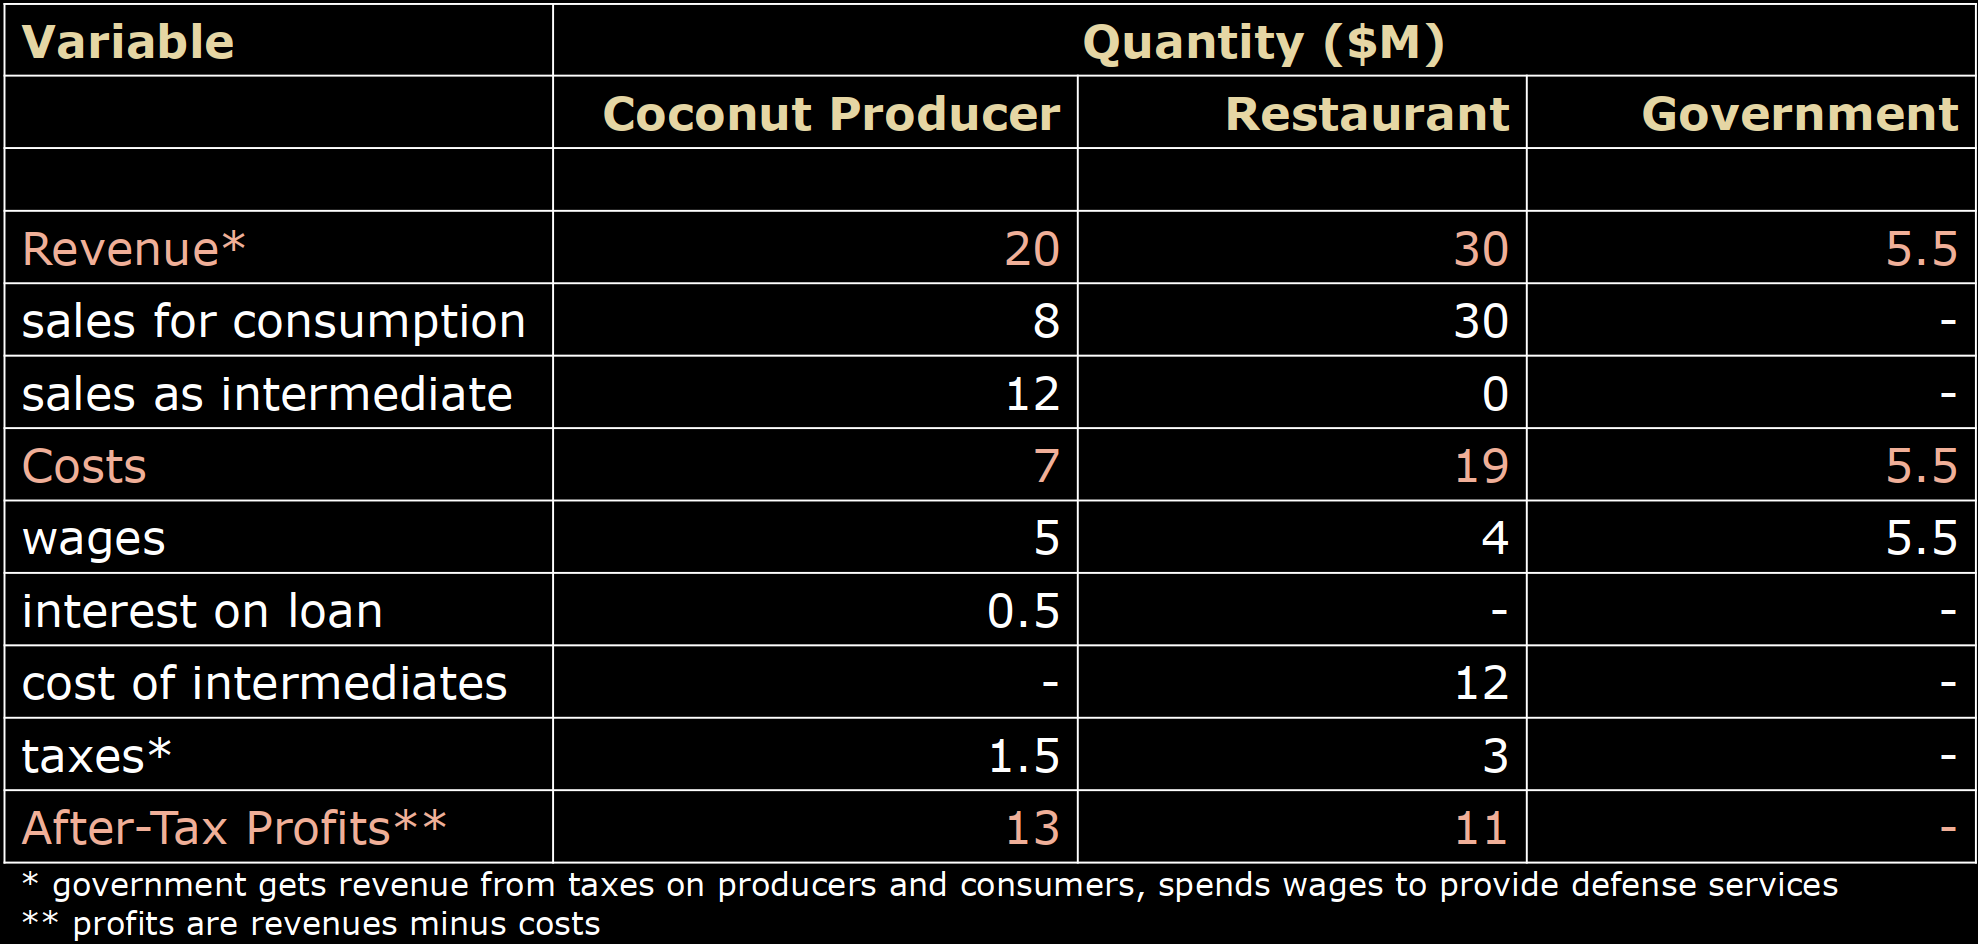
\includegraphics[width=\textwidth]{./figures/ThreeApproachTable1.png}
    \end{figure}
    \alert{Question}: how to calculate GDP?
\end{frame}

\begin{frame}{The Product Approach}
\label{slide:The_Product_Approach}
\textbf{Question}: \alert{What is the value added by each agent?}

\begin{itemize}
    \item \textbf{Coconut Producer}: Final good $ \$20M $, no intermediate input
    \item \textbf{Restaurant}: Final goods $ \$30M $, with intermediate input $ \$12M $ from Coconut Producer
    \begin{itemize}
        \item value added: $ 30 - 12 = 18M $
    \end{itemize}
    \item \textbf{Government}: Defence services, valued at cost $ \$5.5M $
    \item \textbf{GDP}: $ 20 + 18 + 5.5 = 43.5M $
\end{itemize}
\end{frame}

\begin{frame}{The Expenditure Approach}
\label{slide:The_Expenditure_Approach}

\textbf{Question}: \alert{What is the total spending?}

\begin{itemize}
    \item \textbf{Formula}: $ Y = C + I + G + NX $
    \item \textbf{Consumption} ($C$): ``sale for consumption'' row
    \begin{itemize}
        \item To Coconut Producer: $ 8M $
        \item To Restaurant: $ 30M $
    \end{itemize}
    \item No investment ($ I $) and net export ($ NX $).
    \item \textbf{Government} ($G$): defense service $ 5.5M $
    \item \textbf{GDP} ($Y$): $ 38 + 5.5 = 43.5M $
\end{itemize}
\end{frame}

\begin{frame}{Income Approach}
\label{slide:Income_Approach}
    \textbf{Question}: \alert{how much does agent earn?}
    \begin{itemize}
        \item \textbf{Workers}: wages $ 5M $ from Coconut Producer, $ 4M $ from Restaurant and $ 5.5M $ from Government
        \item \textbf{Firms}:
        \begin{itemize}
            \item After-tax Profits: $ 13M $ to Coconut Producer and $ 11M $ to Restaurant
            \item Interest on loan: $ 0.5M $ for Coconut Producer
        \end{itemize}
        \item \textbf{Government}: Taxes $ 1.5M $ from Coconut Producer and $ 3M $ from Restaurant
        \begin{itemize}
            \item Expenditure is $ 5.5M $ $ \Rightarrow  $ \alert{budget deficit}
        \end{itemize}
        \item \textbf{GDP}: $5 + 4 + 5.5 + 13 + 11 + 0.5 + 1.5 + 3 = 43.5M$
    \end{itemize}
    \textbf{Income-Expenditure Identity}: Income earned goes to expenditure
\end{frame}

\section{Inflation}
\label{sec:Inflation}

\begin{frame}{Prices in GDP measurement}
\label{slide:Prices_in_GDP_measurement}
    The \alert{revenue} row is calculated by $ 10M $ coconuts $ \times $ $ \$2 $ each
    \begin{itemize}
        \item What if coconut price increases to $ \$3 $ next year?
    \end{itemize}
    \textbf{Solution}: common \alert{price index} across different time

    Two ways to build common price index:

    \begin{enumerate}
        \item GDP deflator: common \alert{GDP} standard
        \item Consumer Price Index (CPI): common \alert{consumption basket} ($Q$)
    \end{enumerate}
\end{frame}

\begin{frame}{Prices in GDP measurement (Cont.)}
\label{slide:Prices_in_GDP_measurement__Cont__}
    \begin{itemize}
        \item GDP deflator: ratio between nominal and real GDP
        \begin{enumerate}
            \item Calculate real GDP relative to base year by base year \alert{price level}
            \begin{itemize}
                \item E.g. $ RealGDP_{2020} = \text{Cost of } Q_{2020} \text{ at } P_{\alert{2000}} $, use $ 2000 $ as base year
                \item While $ NominalGDP_{2020} = \text{Cost of } Q_{2020} \text{ at } P_{\alert{2020}} $
                \item \alert{Problem}: choose which year? $ \Rightarrow  $ ``\alert{chain-weighting}'' (rolling base)
            \end{itemize}
            \item Calculate ratio: $ \frac{NominalGDP_{2020}}{RealGDP_{2020}} \times 100 $
        \end{enumerate}
        \item CPI: normalize \alert{consumption basket} of \alert{base year} as $ 100 $, relative to \alert{other year}
        \begin{itemize}
            \item E.g. $ CPI_{2020} = \frac{\text{Cost of } Q_{2000} \text{ at } P_{2020}}{\text{Cost of } Q_{2000} \text{ at } P_{2000}} \times 100 $, use $ 2000 $ as base year
            \item \alert{Problem}:
            \begin{enumerate}
                \item $ \Delta P $ outside of consumption basket \&  not accounted
                \item new goods \& services introduced, old goods \& services obsolete
            \end{enumerate}
        \end{itemize}
    \end{itemize}
\end{frame}

\begin{frame}{Example: Nominal v.s. Real GDP}
\label{slide:Example__Nominal_v_s__Real_GDP}
    \begin{itemize}
        \item \textbf{Nominal GDP}: value of goods \& services at current price
        \item \textbf{Real GDP}: value of goods \& services at base year price
    \end{itemize}
    \begin{figure}
        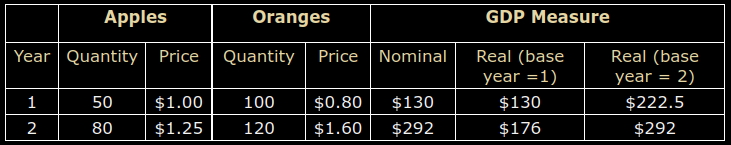
\includegraphics[width=\textwidth]{./figures/GDPMeasurement.png}
    \end{figure}

    Choice of base year affects the GDP measure!

    alternative: chain-weighting

\end{frame}

\begin{frame}{Data: Nominal v.s. Real GDP}
\label{slide:Data__Nominal_v_s__Real_GDP}
    \begin{columns}
        \begin{column}{0.3\textwidth}
            \begin{itemize}
                \item inflation growth $ + $ economics growth $ = $ nominal grows faster than real
                \item \textbf{Question}: \alert{What year is the base year} on this graph?
                \item Ans: 2009, when Nominal $ = $ Real
            \end{itemize}
        \end{column}
        \begin{column}{0.7\textwidth}
            \begin{figure}
                \caption{Figure 2.1 Nominal GDP and Chain-Weighted Real GDP}
                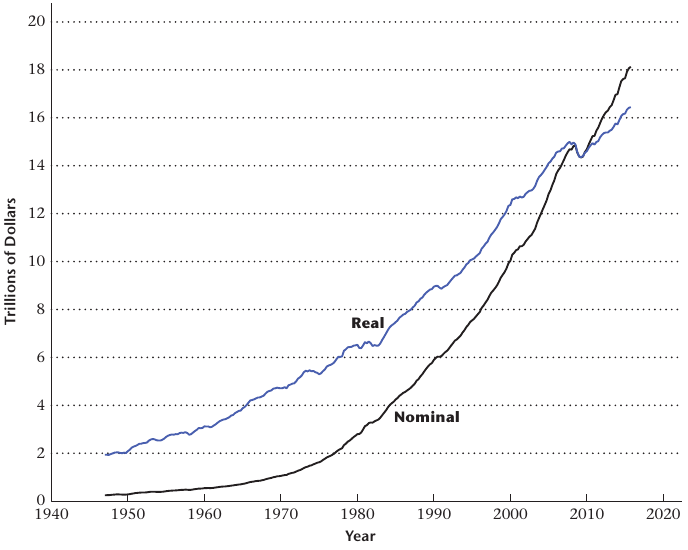
\includegraphics[width=\textwidth]{./figures/Figure2_1.png}
            \end{figure}
        \end{column}
    \end{columns}
\end{frame}

\section{Employment}
\label{sec:Employment}

\begin{frame}{Population Composition}
\label{slide:Population_Composition}
    \hspace{11em} N \hspace{7em} LF \hspace{5em} E/U
    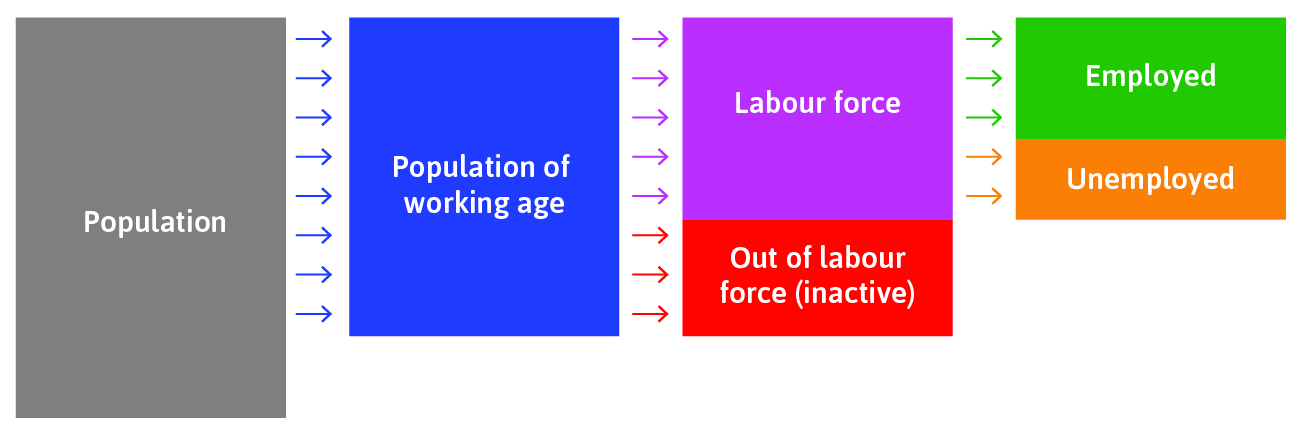
\includegraphics[width=\textwidth]{./figures/employmentPop.jpg}
    \begin{itemize}
        \item participation rate $ = \frac{LF}{N} $
        \item unemployment rate $ = \frac{U}{\alert{LF}} $
        \item employment rate $ = \frac{E}{\alert{N}} $
    \end{itemize}
\end{frame}


\appendix
% -------------------------------------------
\setbeamertemplate{headline}
{
\setbeamercolor{section in head/foot}{fg=black, bg=white}
\vskip1em \tiny \insertsectionnavigationhorizontal{1\paperwidth}{\hspace{0.50\paperwidth}}{}
}
%------------------------------------------
\begin{frame}\frametitle{}
\begin{columns}
\label{Appendix}
\column{1\linewidth}
\centering
{\Large \alert{Appendix}}
\end{columns}
\end{frame}
%------------------------------------------

\begin{frame}{Chain-weighting }
\label{slide:Chain_weighting_}
    Chain
\end{frame}
<++>


\end{document}

